\documentclass[preprint, 1p,
authoryear]{elsarticle} %review=doublespace preprint=single 5p=2 column
%%% Begin My package additions %%%%%%%%%%%%%%%%%%%

\usepackage[hyphens]{url}


\usepackage{graphicx}
%%%%%%%%%%%%%%%% end my additions to header

\usepackage[T1]{fontenc}
\usepackage{lmodern}
\usepackage{amssymb,amsmath}
% TODO: Currently lineno needs to be loaded after amsmath because of conflict
% https://github.com/latex-lineno/lineno/issues/5
\usepackage{lineno} % add
\usepackage{ifxetex,ifluatex}
\usepackage{fixltx2e} % provides \textsubscript
% use upquote if available, for straight quotes in verbatim environments
\IfFileExists{upquote.sty}{\usepackage{upquote}}{}
\ifnum 0\ifxetex 1\fi\ifluatex 1\fi=0 % if pdftex
  \usepackage[utf8]{inputenc}
\else % if luatex or xelatex
  \usepackage{fontspec}
  \ifxetex
    \usepackage{xltxtra,xunicode}
  \fi
  \defaultfontfeatures{Mapping=tex-text,Scale=MatchLowercase}
  \newcommand{\euro}{€}
\fi
% use microtype if available
\IfFileExists{microtype.sty}{\usepackage{microtype}}{}
\usepackage[]{natbib}
\bibliographystyle{plainnat}

\ifxetex
  \usepackage[setpagesize=false, % page size defined by xetex
              unicode=false, % unicode breaks when used with xetex
              xetex]{hyperref}
\else
  \usepackage[unicode=true]{hyperref}
\fi
\hypersetup{breaklinks=true,
            bookmarks=true,
            pdfauthor={},
            pdftitle={From Creators to Adopters. The Role of AI in Driving Economic Growth},
            colorlinks=false,
            urlcolor=blue,
            linkcolor=magenta,
            pdfborder={0 0 0}}

\setcounter{secnumdepth}{5}
% Pandoc toggle for numbering sections (defaults to be off)


% tightlist command for lists without linebreak
\providecommand{\tightlist}{%
  \setlength{\itemsep}{0pt}\setlength{\parskip}{0pt}}







\begin{document}


\begin{frontmatter}

  \title{From Creators to Adopters. The Role of AI in Driving Economic
Growth}
    \author[Hanken School of Economics]{Irina Vélez López%
  \corref{cor1}%
  }
   \ead{irina.velezlopez@student.hanken.fi} 
      \cortext[cor1]{Corresponding author}
    \fntext[1]{Exchange Student.}
  
  \begin{abstract}
  This paper explores the potential of artificial intelligence (AI) and
  Language Models (LLMs) as general-purpose technologies (GPTs) that can
  drive growth and development. AI and LLMs have the capability to
  redefine the ways in which businesses operate, improve productivity,
  and contribute to long-term economic progress. The generalization of
  tools, particularly in the realm of AI, enhances the potential for
  productivity improvements and opens up new possibilities for value
  creation. However, the coexistence of forward-looking optimism and
  backward-looking disappointment is a natural aspect of transformative
  periods. Grounded expectations are crucial in these periods, as there
  can be a discrepancy between optimistic expectations and actual
  outcomes. The integration of new technologies takes time, and creators
  and adopters play a critical role in realizing the potential benefits
  of AI. It concludes by highlighting the importance of grounded
  expectations and the value of intangible assets in the process of
  economic transition.
  \end{abstract}
    \begin{keyword}
    General Purpose Technology \sep Artificial Intelligence \sep 
    Creative destruction
  \end{keyword}
  
 \end{frontmatter}

\hypertarget{introduction}{%
\section{Introduction}\label{introduction}}

The generalization of tools is a crucial factor in harnessing the
potential for growth and development. When a tool can be widely used for
various purposes, its value increases significantly. In the realm of
artificial intelligence (AI), Language Models (LLMs) serve as a
foundational technology for other tools, such as AI-powered software.
This opens up new possibilities and enhances the potential for
productivity improvements in the workforce. As mentioned by
\citep{gptaregpts}, LLMs like Generative Pre-Trained Transformers (GPTs)
exhibit characteristics of general-purpose technologies, which can have
profound economic, social, and policy implications.

The emergence of new capabilities and the widespread adoption of LLMs as
enablers of new AI-based tools, coupled with the increasing number of
users utilizing tools like ChatGPT, signifies a future that has not been
seen before. This accelerated expansion and pushing of boundaries and
limits hold the potential for transformative changes.

In light of these dynamics, it is important to recognize that while
there may be optimism surrounding new technologies, there can also be a
discrepancy between expectations and actual outcomes. This coexistence
of forward-looking optimism and backward-looking disappointment is a
natural aspect of periods of transformative change. It reflects the
human desire to witness the fulfillment of expectations within their
lifetime, while also acknowledging the time required for society to
fully integrate and benefit from these innovations.

\hypertarget{general-purpose-technology-ai-and-large-language-models}{%
\section{General Purpose Technology, AI, and Large Language
Models}\label{general-purpose-technology-ai-and-large-language-models}}

General Purpose Technology is a transformative technology with a strong
improvement process at the begining and eventually becoming widely
adopted for its multiples uses, while producing many spillover effects
\citep{paradox}. As such, it have a pervasive impact on society as a
whole, mainly due to its capability to redefine the ways in which
businesses operate, improve productive and contribute to long-term
economic growth. Some well-know examples are steam power, electricity,
semiconductors, and internet.

Most GPTs play the role of enabling technologies, opening up new
opportunities rather than offering complete, final solutions
\citep{enginesofgrowth}. Therefore, their contribution depends on the
ability to successfully use GPTs as enablers. The generic function or
general concept behind AI is to simulate human cognitive abilities,
which can be applied in many sectors.

Artificial intelligence a term coined by emeritus Stanford Professor
John McCarthy in 1955, was defined by him as ``the science and
engineering of making intelligent machines''.\footnote{Available at:
  \url{https://hai.stanford.edu/sites/default/files/2020-09/AI-Definitions-HAI.pdf}}
These systems are designed to simulate human cognitive abilities, such
as learning, reasoning, problem-solving, perception, and language
understanding. Within the realm of AI, Large Language Models (LLMs) are
a specific type of AI model that utilizes deep learning techniques,
particularly neural networks, to process and generate human-like
language. LLMs are trained on vast amounts of text data and can perform
tasks like language translation, text summarization, and question
answering.

In the past, computer programs were developed by painstakingly encoding
human knowledge, following a precise set of instructions that mapped
specific inputs to desired outputs. This approach required programmers
to meticulously define every step of the process. However, machine
learning systems operate differently. They utilize general algorithms,
such as neural networks, which enable them to independently determine
the appropriate mapping between inputs and outputs. This is achieved
through exposure to extensive datasets containing numerous examples. By
analyzing and learning from these examples, machine learning systems can
identify patterns and make accurate predictions or classifications
without explicit programming instructions.

\hypertarget{key-factors-contributing-to-the-widespread-adoption-of-a-technology-as-a-gpt}{%
\subsection{Key factors contributing to the widespread adoption of a
technology as a
GPT}\label{key-factors-contributing-to-the-widespread-adoption-of-a-technology-as-a-gpt}}

In the case of LLMs, emergent abilities such as text understanding,
generation, problem-solving, mathematics, and data classification have
arisen due to the increased computational power required to train these
models (10\^{}23 training FLOPs). As research progresses, understanding
how emergence occurs in LLMs could provide new insights into training
more-capable language models. This emergence of new abilities is one of
the key factors in the widespread adoption of LLMs as a GPT.

AI as a General Purpose Technology has transformative potential,
versatility, and wide-ranging applicability across various sectors and
industries. By simulating human cognitive abilities, AI systems can
tackle complex tasks and make accurate predictions or classifications.
AI's scalability, adaptability, and capacity to integrate with other
technologies enhance its impact and expand its applications.

\hypertarget{what-is-the-potential-economic-impact-of-ai}{%
\section{What is the potential economic impact of
AI?}\label{what-is-the-potential-economic-impact-of-ai}}

Considering the AI as a new General Purpose Technology, assessing its
possible contribution to economic growth is worthwhile in times of
dizzying change such as the present. The winds of uncertainty are
blowing everywhere and it would be useful to set expectations. Given the
conditions of uncertainty and the low accuracy of predictions, the
assessment of its potential impact seems to be addressed only by a
retrospective approach, which means that the performance of previous
general-purpose technologies, such as steam power, electricity or the
Internet, could provide a more realistic answer to this question.

However, this topic has already been addressed by \citep{paradox} and
\citep{Nicholas}, in a context where there are optimists and pessimists
about technology and growth. A real dichotomy emerges between the higher
profit expectations of forward-looking entrepreneurs and the poor growth
performance reflected in retrospective statistics.

One example mentioned by \citep{paradox} is the call center industry,
which had approximately 2.2 million agents in 2015 in the United States.
It was plausible at that time to anticipate that voice recognition
systems like IBM's Watson could potentially reduce the number of workers
by 60\%. However, in hindsight, it is evident that the expectations have
not been fully met, as shown in Figure \ref{fig1}, which illustrates the
statistics.

\begin{figure}

{\centering 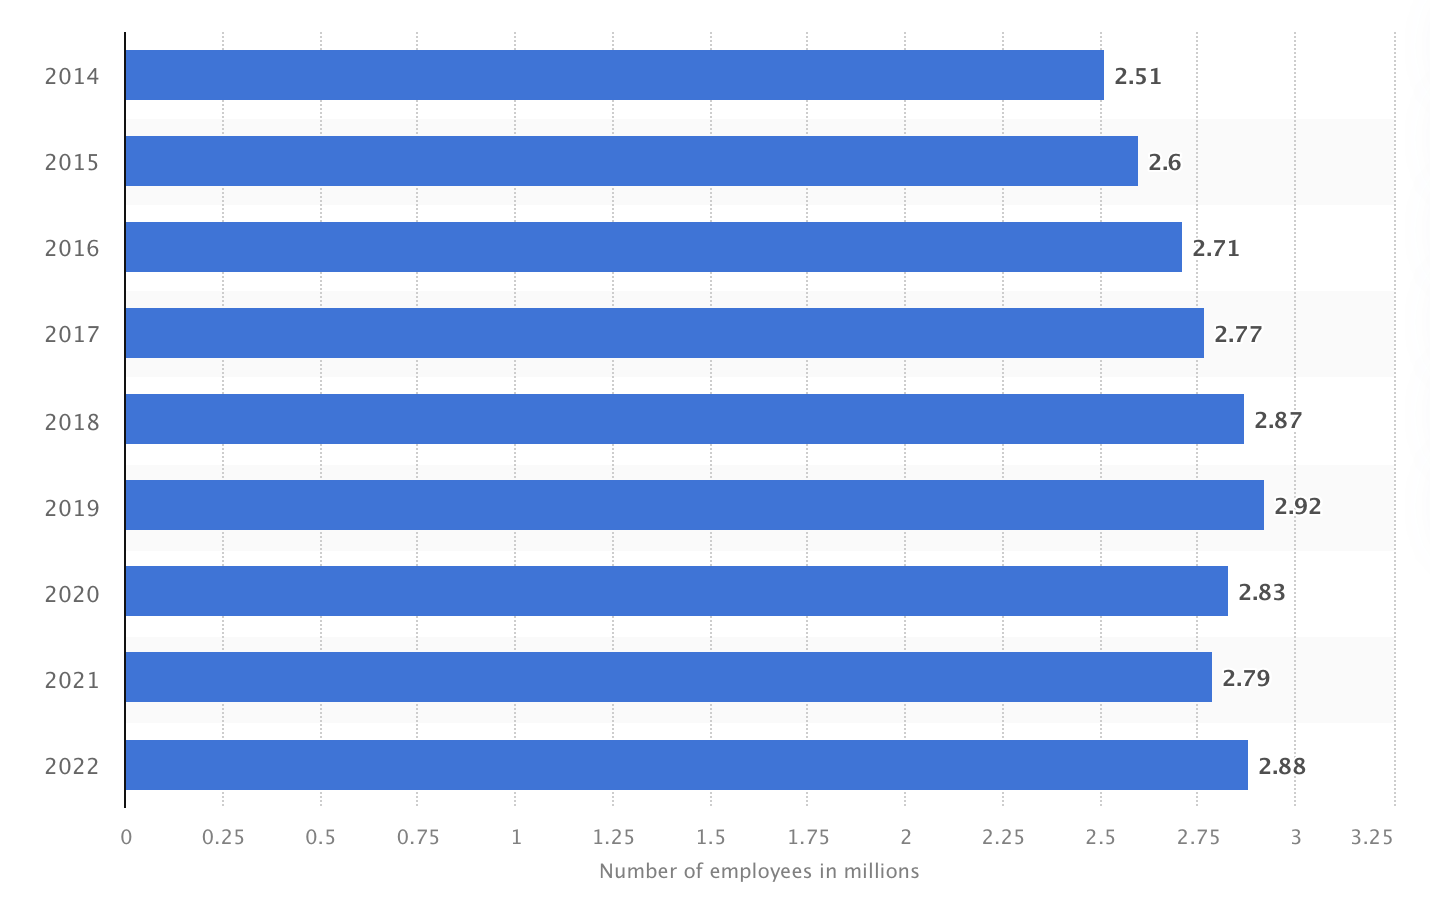
\includegraphics[width=0.7\linewidth]{../Views/contact_center_employees_US} 

}

\caption{\label{fig1}Number on contact center employees in the United States from 2014 to 2022.}\label{fig:fig1}
\end{figure}

As \citep{paradox} explains, this apparent incongruity is due to the
time lag between the creation of the technology and the full realization
of its benefits in the economy and society. It takes time to build up
the stock of the new technology, develop the necessary human capital
skill set, undergo the process of re-engineering business process
transformations, and develop complementary innovations for full
realization in the real economy.

To support this explanation of the lag, the Schumpeterian growth model
could offer a good perspective, taking as a starting point that the real
contributions to growth are value creation and cost optimization, so AI
should serve these growth contributors.

\hypertarget{assessing-the-potential-economic-impact-of-ai-in-terms-of-value-creation-and-cost-optimization.}{%
\subsection{Assessing the potential economic impact of AI in terms of
value creation and cost
optimization.}\label{assessing-the-potential-economic-impact-of-ai-in-terms-of-value-creation-and-cost-optimization.}}

From an economic perspective, one of the fundamental problems in
understanding corporate behavior is the pursuit of profit maximization
by firms. This objective drives economic growth and leads to two main
objectives in the private business sector: adjusting the production
function to obtain the right quantities to supply the market, while
coping with constraints, often in the form of a limited budget.

The firm's goal of maximizing profits can be represented as follows: \[
Profit = Total \ Income - Total \ Costs: \Pi = PX - C(X)
\] \[
Maximization \ Problem: \max_{x} \Pi(X) = PX - (wL + rK)
\]

Where PX represents the revenue generated by production function X, and
C(X) represents the corresponding costs associated with labor and
capital costs. Thus, on one side of the coin, value creation contributes
to increasing profits by adjusting the output of production function X,
while on the other side, cost optimization aims to mitigate not only
budget constraints but also resource constraints. Therefore, AI must be
oriented towards achieving one or both of these objectives to promote
growth.

To exemplify value creation through AI, consider the use of deep neural
network systems in skin cancer diagnosis \citep{cancer}, fraud detection
and risk assessment in the financial sector, and inventory forecasting
automation, as seen in Amazon's AI-powered inventory management product.
On the other hand, from a cost optimization perspective, AI is used in
predictive maintenance and quality control to anticipate equipment
failures\footnote{Available at:
  \url{https://www.ge.com/research/project/predictive-maintenance}}.

\hypertarget{shumpenters-concept-of-creative-destruction}{%
\subsection{Shumpenter's concept of creative
destruction}\label{shumpenters-concept-of-creative-destruction}}

Creative destruction refers to the process of creating and developing
new technology that continuously disrupt and replace the existing
obsolete technology in order to drive economic progress and growth.

Thus, let us consider two types of companies, those that are creators of
new technologies and major investors in R\&D, such as big technology
companies like Apple, Amazon, Meta or Google, called ``creators'' of
technology, and on the other hand, companies that adopt and implement
the new technology released by the creators, called ``adopters'' of
technology.

In addition, knowledge or innovation is considered a \textbf{public
good}, one you have invented something , it is almost free to spread it
around the world. Thus, the first initial cost of producing the
technology has to be covered through monopoly profits (Creators),
because this has been the mechanism that the market system has found to
cover the huge initial costs\footnote{Insights taken from this
  \href{https://youtu.be/m3nkTrFF2zs?si=dgPJlvVgQuuQAcL8}{Bilkent
  Üniversitesi lecture}}.

Once the new technology has been widely launched in the market at an
almost affordable or even free price, as in the case of ChatGPT, the
maturity level or readiness of the adopter must be high in order to take
advantage of the full potential of the new technology. From the
adopter's point of view, it takes time to evolve and incorporate the new
technology into their business process in a way that is effective and
beneficial to the business. This evolution requires developing new
business processes, adjusting their production functions to add value to
their bottom line, and reallocating skilled human capital to address the
transformation.

Destruction is represented in the Schumpeterian Growth Model as the
expected years that firms will remain in the market, if they do not
adapt. And this adaptation process is mainly promoted by the creation of
new ideas E{[}A{]}. This time expectation is represented by the
following equation

\[
Firm \ Lifetime: E[\tau] = 1/E[A]
\] \[
Firm \ Lifetime: E[\tau] = 1/\gamma N
\] Where: New ideas corresponds to \(E[A] = \gamma N\)

The life of the company is reduced by the increase in productivity
(\(\gamma\)) and the deployment of new technologies (N). This leads to
two transition scenarios

\begin{enumerate}
\def\labelenumi{\arabic{enumi}.}
\item
  If the adopter is not able to incorporate the new technologies or take
  advantage of them, its profit will be decreasing until a possible exit
  from the market, when its profits will be zero, and therefore, this
  company will not contribute to the growth of the economy.
\item
  If the adopting company is able to incorporate the new technology or
  take advantage of it, its profit will increase, which in turn will
  ensure its permanence in the market. However, this benefit is not
  immediately reflected in the aggregate accounting statistics. The
  process of adaptation takes time, due to the development of new
  business processes, the upgrading of the skills of its human capital,
  the time required for the reallocation of more qualified human capital
  from less capable firms to firms with more potential for growth or
  success.
\end{enumerate}

This reallocation of human capital can be seen in one of the key
statistics in the labor market: Job postings.The number of AI related
job postings has increased on average from 1.7\% in 2021 to 1.9\% in
2022 according to \citep{reportAI}. This increased trend can be seen in
Figure \ref{fig2}. In 2022, the top three countries with the higher
percentage of AI job postings were the United States (2.1\%), Canada
(1.5\%), and Spain (1.3\%).

\begin{figure}

{\centering 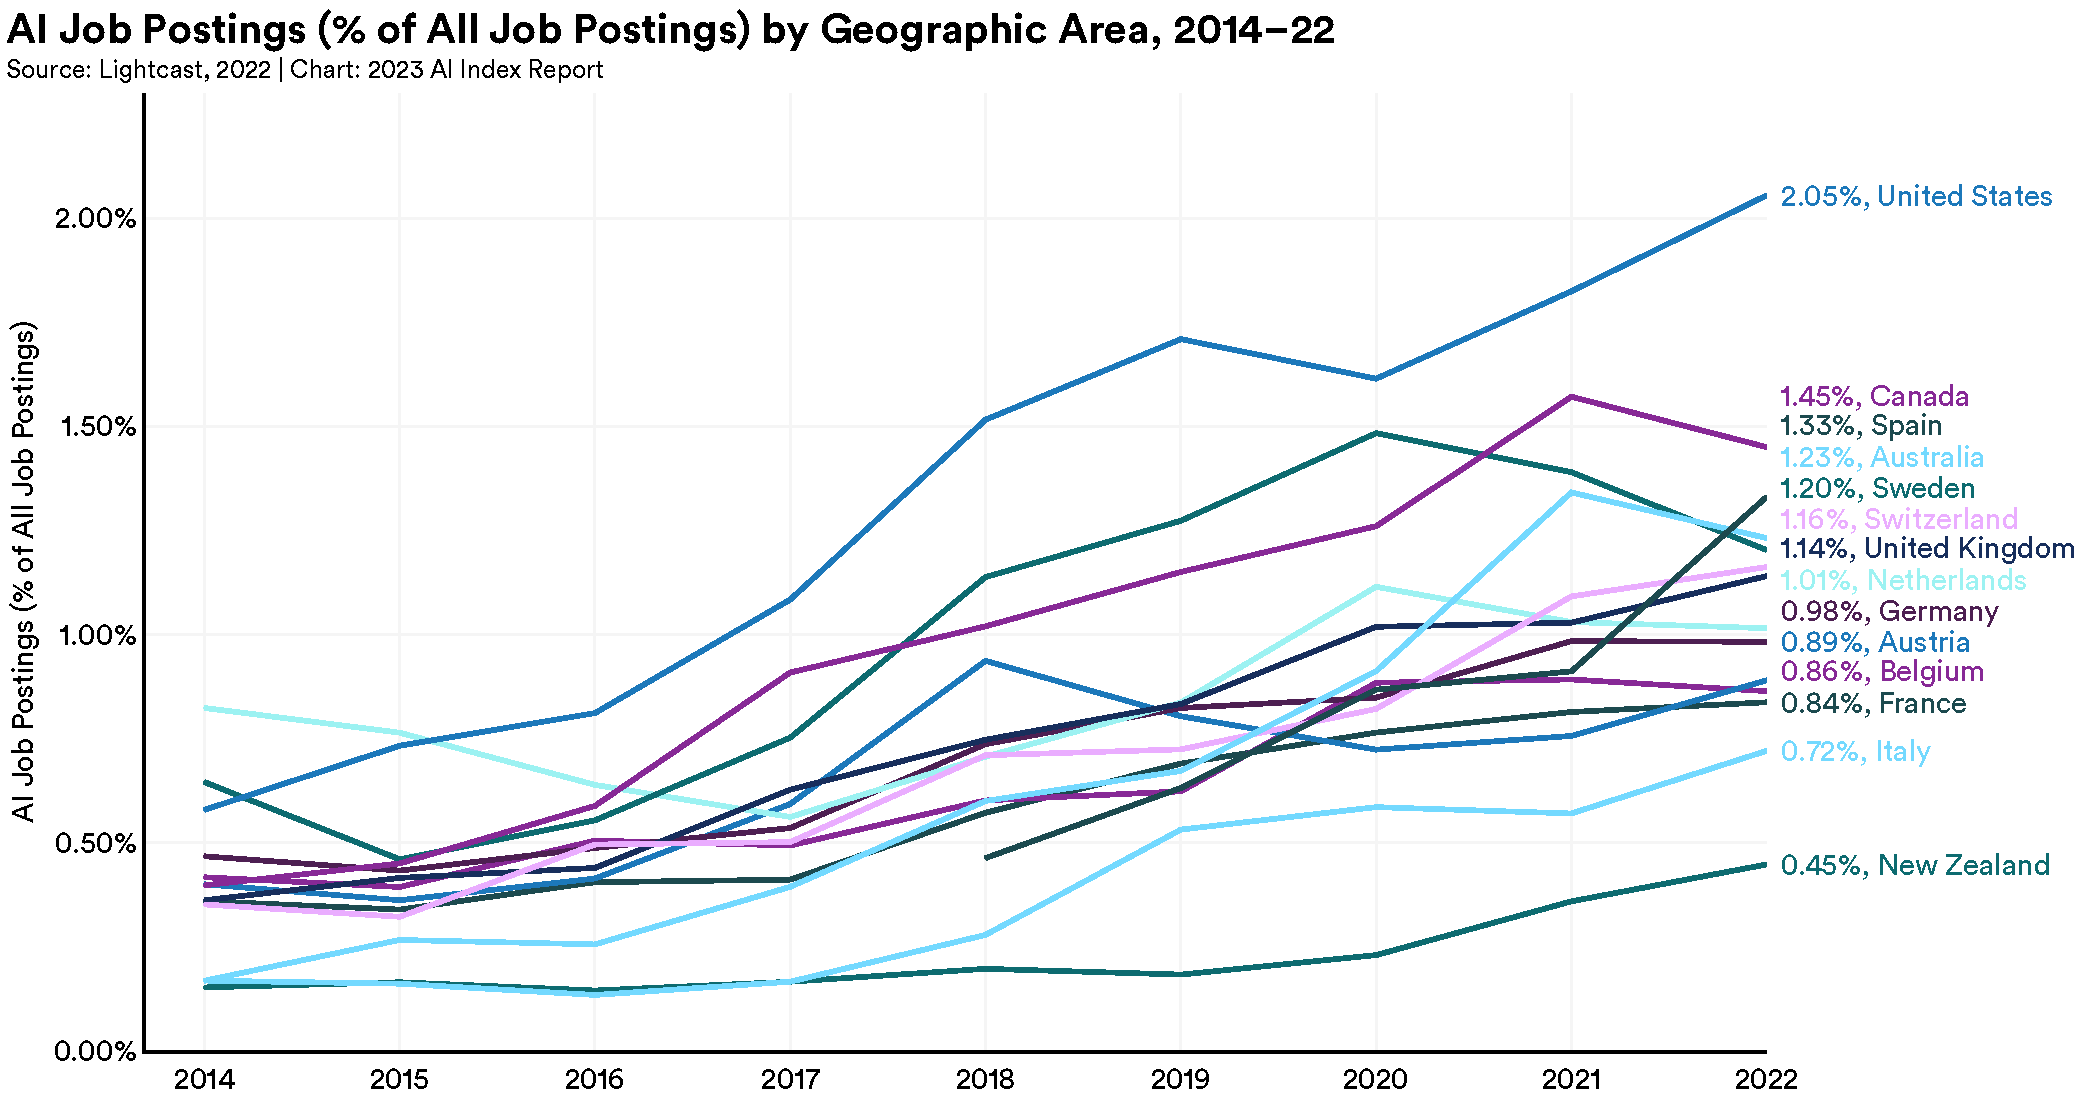
\includegraphics[width=0.7\linewidth]{../Views/AI_job_postings_by_geo_area} 

}

\caption{\label{fig2} Percentage of all job postings that require some kind of AI skill by Geographic Area, 2014 to 2022.}\label{fig:fig2}
\end{figure}

Thus, in times of structural change like the present, it is challenging
to observe the results of new technologies, as the contributions to
growth made by successful firms are often offset by the declining
profits of firms in decline. Therefore, it is reasonable to think that
current statistics may not yet reflect the potential benefits of using
AI.

This can be illustrated by reviewing the investments in AI over the last
decade and the historical behavior of the Multiple Factor of
Productivity.

Figure \ref{fig3} shows an upward trend in global AI investments over
the last decade, with the exception of 2022, when, for the first time
since 2013, global business investment in AI has declined.

However, these investments have not yet translated into increases in the
Multi Factor of Productivity (MFP), as can be seen in Figure \ref{fig4}
and Figure \ref{fig5}.

Figure \ref{fig4} shows a decreasing trend in MFP since 1996, while
Figure \ref{fig5} shows the average behavior of the MFP by continent.
Despite investments in AI since 2013, this trend has not changed.
Therefore, this is an indicator that new technologies such as AI may not
yet have reflected their benefits in the economy.

\begin{figure}

{\centering 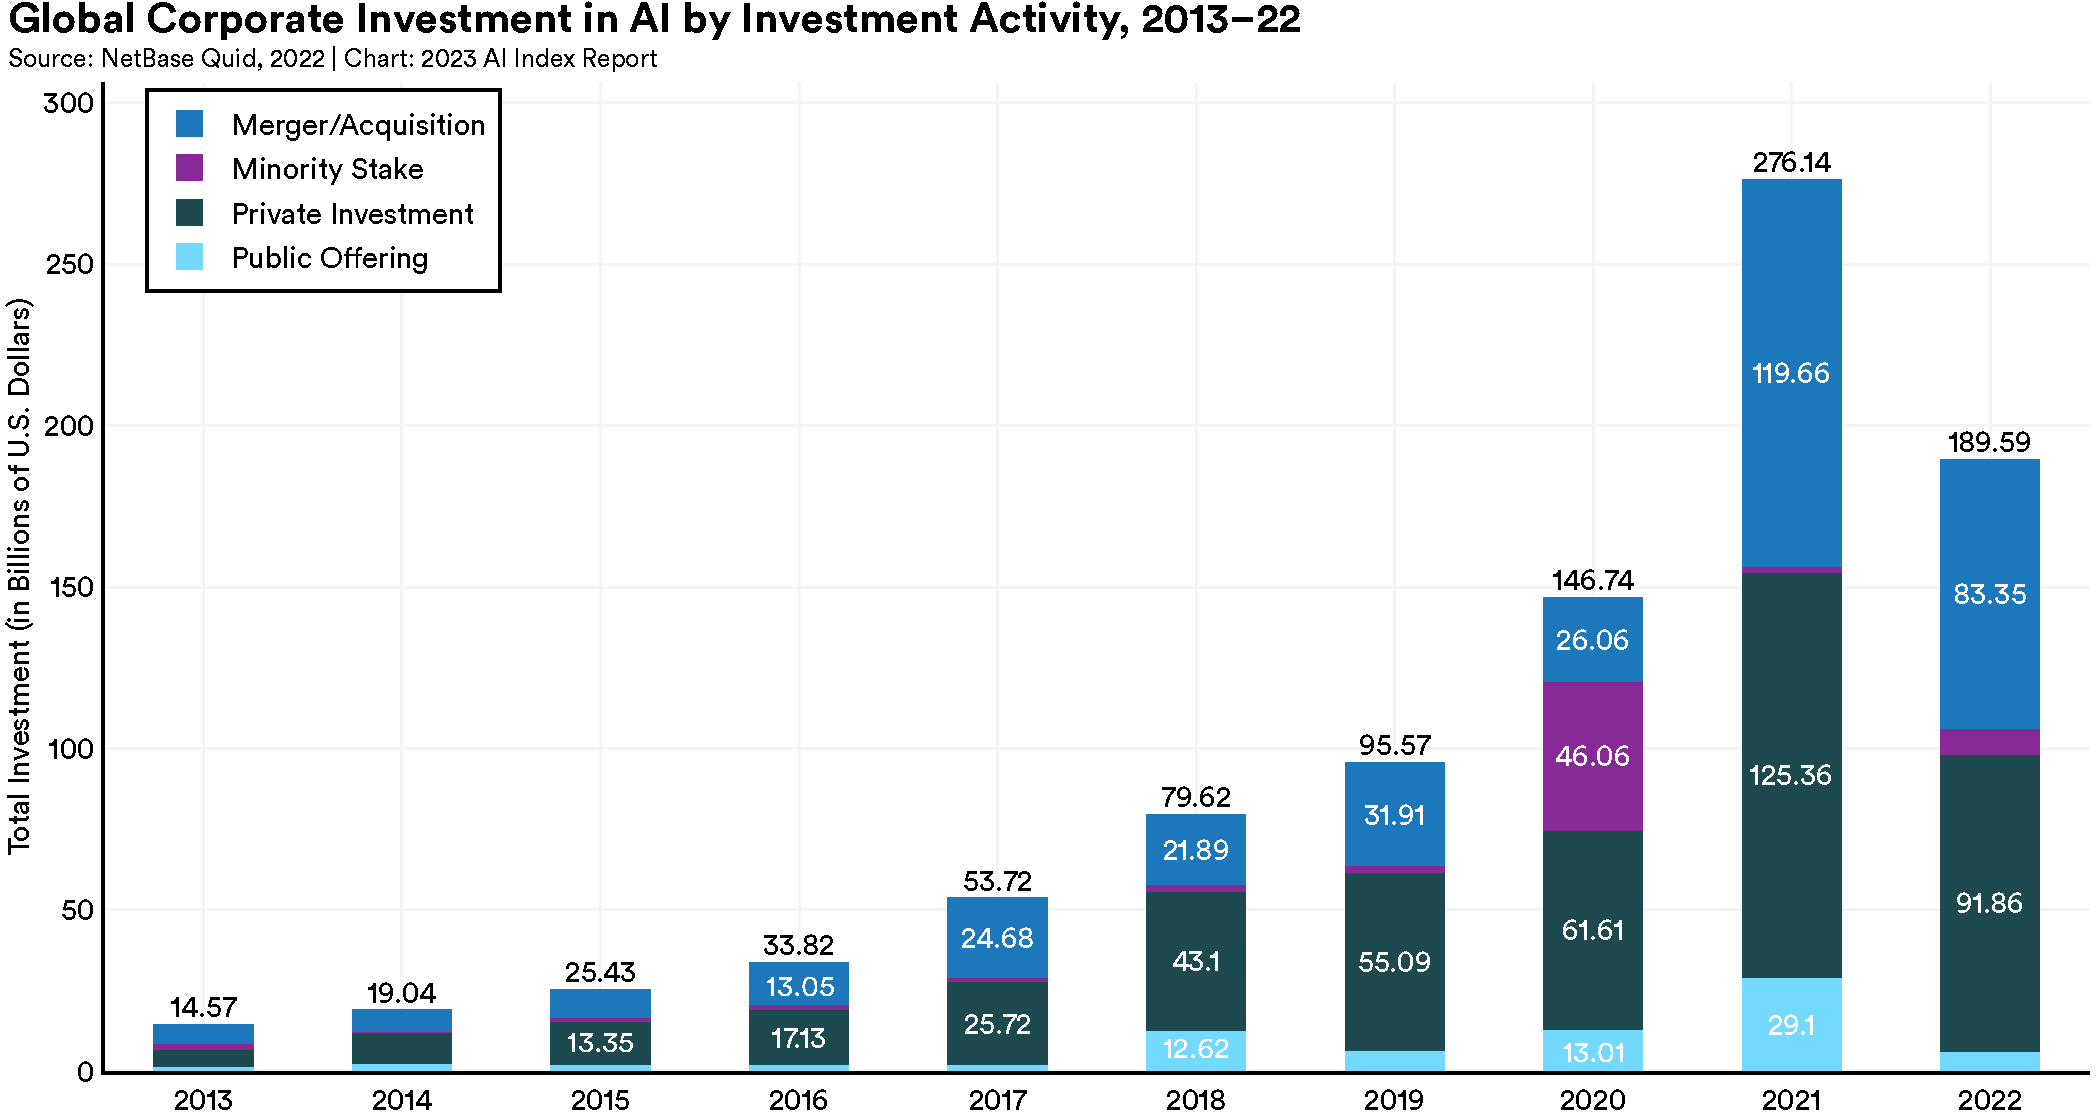
\includegraphics[width=0.7\linewidth]{../Views/global_investiment_by_inv_activity} 

}

\caption{\label{fig3}Global Corporate Investment in AI by Investment Activity, 2013 to 2022.}\label{fig:fig3}
\end{figure}

\begin{figure}

{\centering 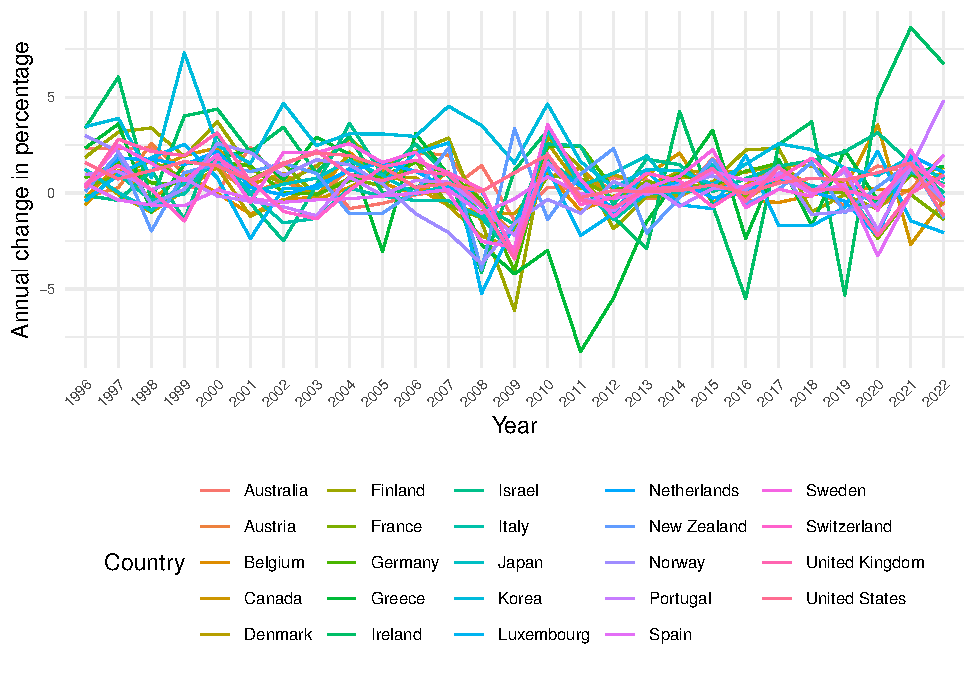
\includegraphics[width=0.8\linewidth]{Document_files/figure-latex/fig4-1} 

}

\caption{\label{fig5}Mean and median Multifactor Productivity per year for OECD countries, 1996 to 2022. The dashed black lines represent the mean and median trend line}\label{fig:fig4}
\end{figure}

\begin{figure}

{\centering 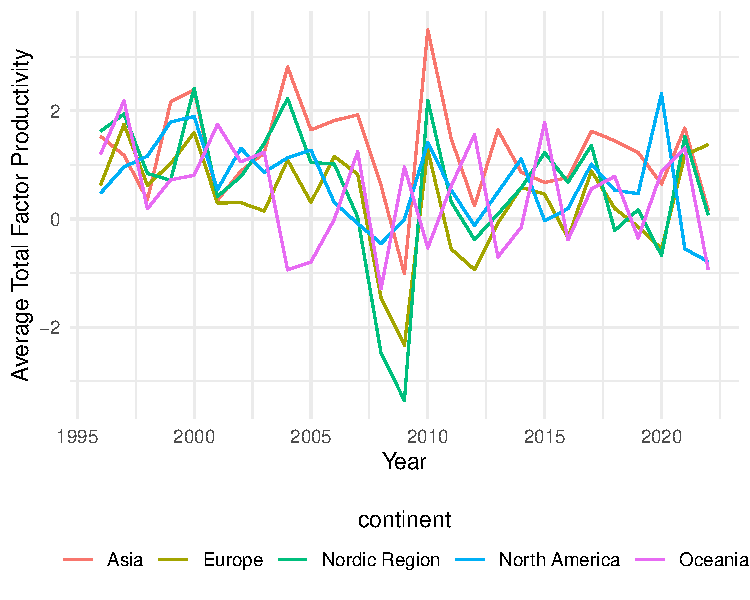
\includegraphics[width=0.8\linewidth]{Document_files/figure-latex/fig5-1} 

}

\caption{\label{fig4}Average of Multi Factor Productivity by Continent, 1996 to 2022.}\label{fig:fig5}
\end{figure}

Nevertheless, this result may not be entirely accurate, as the
measurement tools available to us today may not be capturing the real
impact of these technologies. Mainly because multifactor productivity
growth is measured as a residual, i.e., the part of GDP growth that
cannot be explained by growth in labor and capital inputs.Traditionally,
TFP growth has been considered to reflect technological progress, but in
practice this does not mean that this parameter reflects all the
benefits.

However, in aggregated terms or in a wide country perspective, Multi
Factor of Productivity is a good approach to assess the technological
contribution. MFP also captures other factors, such as adjustment costs,
economies of scale, and effects from imperfect competition.

\hypertarget{a-country-level-perspective-creators-and-adopters}{%
\subsection{A country-level perspective: Creators and
Adopters}\label{a-country-level-perspective-creators-and-adopters}}

To ilustrate better the concept of creative destruction and its
challenges measuring the economic impact of AI, let's consider a country
like Colombia. Suppose that Colombia has a fixed amount of resources, R,
that it can allocate towards different economic activities. The country
can divide these resources in the following way:

Creators: Proportion n does R\&D: \(nR\). A proportion n of the
resources are allocated towards Research and Development (R\&D)
activities. R\&D is the process of creating new knowledge and
technologies that can be used to improve productivity and create new
products and services. Examples of R\&D activities include developing
new AI algorithms, creating new software, and conducting experiments to
test new business models.

Adopters: The remainder goes to produce X: \((1-n)R\), are allocated
towards producing a certain level of product or result X. Adopters are
individuals or firms who use existing technologies to produce goods and
services. While they may not be involved in creating new technologies,
they play a critical role in bringing new products and services to
market.

Those resources are organized by companies as a composite of human
capital, creators are individuals with the necessary skills to create
new technologies and a deep understanding of the underlying
technologies, while adopters are individuals with sufficient skills to
produce X in the traditional business model. Now, adopters need to
acquire new skills in order to incorporate the benefits of technology,
creating new business processes and successfully transitioning their
production from the old schemes to the new schemes. These adopters are
investing in intangible assets that the metrics are not reflecting. More
importantly, adopters need the help of creators to facilitate the
adoption process in their industries, because it stands to reason that
creators are the most skilled human capital part of the available
resources.

At the firm level, adapting firms can benefit from adopting a similar
approach to resource allocation. Firms that allocate a portion of their
resources towards R\&D are more likely to be successful in transitioning
to a new business model. In practical terms, from the perspective of an
adopting company:

Business Transformers: The ratio n avoids exiting the market and are
responsible for leading the firm's successful transition to a new
business mode: \(nR\). Change assimilators: This ratio continues to
maximize profit in the new business model: \((1-n)R\).

Since consumers are not part of the production process, they have been
left out of this analysis. However, their acceptance towards the
consumption of AI-based products and their expected increase in the
consumption of AI-based services will have a positive impact on economic
growth.

It is important to note that there are intangible assets associated with
the transformation process that are not yet quantified. In the last wave
of computerization, the value of these intangibles was about ten times
greater than the direct investments in computer hardware
\citep{paradox}. Given the complexity and novelty of AI-based
technologies, it is plausible that the intangibles associated with AI
are of comparable or greater magnitude. Examples of intangible assets
associated with AI include data, algorithms, access to massive data,
training and organizational capabilities.

\hypertarget{conclusion}{%
\section{Conclusion}\label{conclusion}}

The positive expectations surrounding new technologies, such as AI, are
often accompanied by optimism from industry leaders, technology experts,
and venture capitalists, leading to speculative investments and
forecasts of future corporate wealth in the financial sector. However,
as (Brynjolfsson et al., 2017) suggest, there is no inherent
contradiction between forward-looking technology optimism and
backward-looking disappointment. The two can coexist, especially in
periods of transformational change, due to human nature, as individuals
want to see their expectations fulfilled throughout their lives. But the
time it takes for society to fully incorporate and benefit from new
technologies could be longer, resulting in a slower rate of
assimilation.

Although I am not concluding anything new to what has been mentioned
before by several authors, it has been worthwhile to review especially
the position of \citep{paradox} from the vision of the Schumpeterian
growth model, and some metrics such as the Multifactor productivity and
investments in AI, which allow us to have more grounded expectations of
these new technologies. I have also emphasized the value of intangible
assets that are part of the economic transition process.

While optimism and speculation around new technologies are common, it is
essential to approach them with a nuanced understanding of the
complexities and challenges of economic transition. By considering both
the tangible and intangible aspects of this process, we can better
understand the potential benefits and limitations of new technologies
and make informed decisions about their adoption, implications and
integration into society.

\renewcommand\refname{References}
\bibliography{mybibfile.bib}


\end{document}
